% IMPORTANT! In order for the document to compile, one needs to use XeLaTeX or LuaLaTeX as compiler. This can be done in  Overleaf by Menu -> Settings -> Compiler -> Choose XeLaTeX/LuaLaTeX
\documentclass[t,24pt,aspectratio=169]{beamer}

\usepackage{KUstyle}
\usepackage[style=authortitle,backend=biber]{biblatex}
\usepackage[]{float}
\usepackage{multicol} % Package for multiple coloumns
\usepackage{listings} % Package for code snippets
\usepackage{amsmath}
\usepackage{stmaryrd}

\newcommand{\cleftsemicirc}{\put(3.5,2.5){\oval(5,10)[l]}\put(3.5,-2.5){\line(0,0){10}}\phantom{\circ}}
\newcommand{\crightsemicirc}{\put(1.5,2.5){\oval(5,10)[r]}\put(1.5,-2.5){\line(0,0){10}}\phantom{\circ}}
\newcommand{\hole}{\cleftsemicirc \crightsemicirc}
\newcommand{\enc}[1]{\llbracket #1 \rrbracket}
\newcommand{\conf}[2]{\langle #1,#2 \rangle}

\lstset{basicstyle=\footnotesize\ttfamily,breaklines=true}
\lstset{frame=single}
\lstset{escapeinside={<@}{@>}}

\addbibresource{../report/references/ref.bib}


%\toplinje{Master's thesis} % The text at top. Remove the command if no text is desired

\begin{document}

% The first slide. One can for instance change the main title, the subtitle, speaker, KU-unit and date
{
\setbeamertemplate{background}{
\includegraphics[width=\paperwidth,height=\paperheight]{KU/forside.pdf}}
\begin{frame}
    \begin{textblock*}{\textwidth}(0\textwidth,0.1\textheight)
        \begin{beamercolorbox}[wd=7.8cm,ht=7.3cm,sep=0.5cm]{hvidbox}
            \fontsize{5}{10}\fontfamily{ptm}\selectfont \textls[200]{UNIVERSITY OF COPENHAGEN}
            \noindent\textcolor{KUrod}{\rule{6.8cm}{0.4pt}}
        \end{beamercolorbox}
    \end{textblock*}
    \begin{textblock*}{\textwidth}(0\textwidth,0.1\textheight)
        \begin{beamercolorbox}[wd=7.8cm,sep=0.5cm]{hvidbox}
            \Huge \textcolor{KUrod}{Master's thesis}
            \vspace{0.5cm}
            \par
            \Large Implementation of a type-safe
            generalized syntax-directed editor
            \vspace{0.5cm}
            \par
            \normalsize Sune Skaanning Engtorp
            \vspace{0.3cm}
            \par
            \footnotesize Advisor: Hans Hüttel
        \end{beamercolorbox}
    \end{textblock*}
    \begin{textblock}{1}(6.3,11.38)
        
\includegraphics[width=1cm]{KU/KU-logo.png}
    \end{textblock}
\end{frame}
}

\begin{frame}[hvid]
    \frametitle{Agenda}

    \begin{itemize}
        \item Motivation
        \item Goal of the project
        \item Background
        \item Implementation
        \item Editor examples
        \item Conclusion
        \item Questions
    \end{itemize}
\end{frame}

\begin{frame}[hvid]
    \frametitle{Motivation}
    \begin{itemize}
        \item Structure editors
              \begin{itemize}
                  \pause
                  \item Avoid syntax errors
                        \pause
                  \item (Arguably) Improved code overview
                        \pause
                  \item With ability to support
                        \begin{itemize}
                            \pause
                            \item Typed holes
                                  \pause
                            \item Context-sensitive syntax
                        \end{itemize}
              \end{itemize}
    \end{itemize}
\end{frame}


\begin{frame}[hvid]
    \frametitle{Motivation (Continued)}

    \begin{multicols}{2}
        \begin{itemize}
            \item Cornell Program Synthesizer (1981)\footcite{timtom81}

        \end{itemize}
        \vfill\null
        \columnbreak
        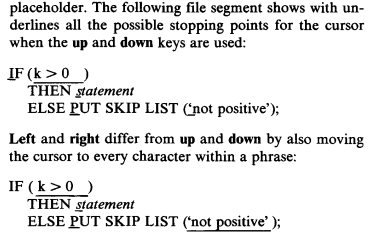
\includegraphics[width=0.4\textwidth]{img/cornell-ex.png}
    \end{multicols}
\end{frame}

\begin{frame}[hvid]
    \frametitle{Motivation (Continued)}

    \begin{multicols}{2}
        \begin{itemize}
            \item Hazel programming environment (2019)\footcite{omar}

        \end{itemize}

        \columnbreak
        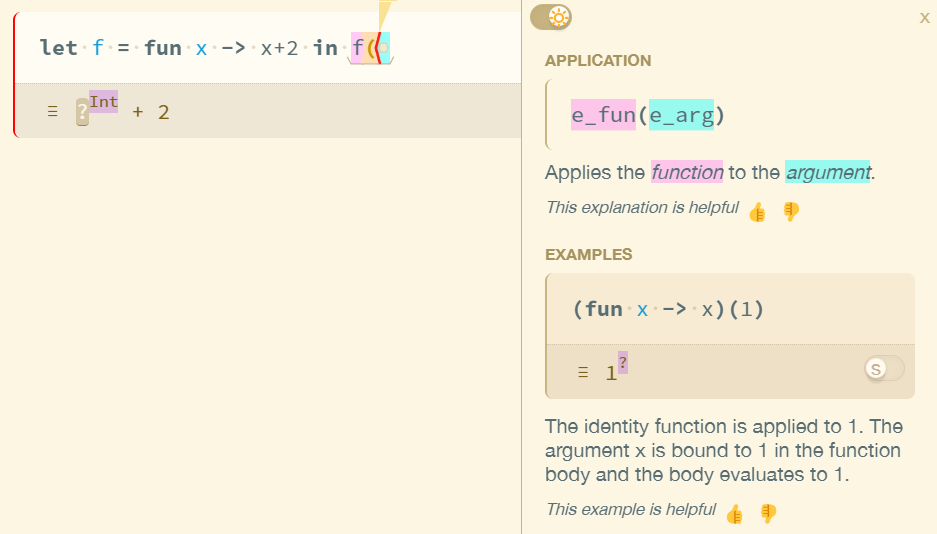
\includegraphics[width=0.5\textwidth]{img/hazel-ex.png}
    \end{multicols}
\end{frame}

\begin{frame}[hvid]
    \frametitle{Motivation (Continued)}

    \begin{multicols}{2}
        \begin{itemize}
            \item<1-> Type-Safe Structure Editor Calculus\footcite{godiksen}
            \item<2-> Implemented by a group of UCPH students\footcite{KU-bach}
            \item<3-> Generalized by a group of AAU students\footcite{aalborg}

        \end{itemize}

        \columnbreak
        \includegraphics<2->[width=0.5\textwidth]{img/ku-editor-ex.png}
    \end{multicols}
\end{frame}

\begin{frame}[hvid]
    \frametitle{Goal of the Project}
    \setbeamercovered{transparent}
    \begin{itemize}
        \item Implement an editor based on the generalized calculus
        \item Criteria for a good implementation:
              \begin{itemize}
                  \pause
                  \item Editing the abstract syntax of any program directly
                        \pause
                  \item Generic editing
                        \pause
                  \item Handling context-sensitive syntax
                        \pause
                  \item Multiple views of code being edited
                        \pause
                  \item Non-challenging way of specifying syntax
              \end{itemize}
              \pause
        \item Minimum viable product:
              \begin{itemize}
                  \pause
                  \item Editing the abstract syntax of any program directly
                        \pause
                  \item Generic editing
              \end{itemize}

    \end{itemize}
    \setbeamercovered{invisible}
\end{frame}

\begin{frame}[hvid]
    \frametitle{Picking good language examples}
    \begin{itemize}
        \item What makes a good set of examples?
              \begin{itemize}
                  \item Different paradigms and purposes:
                        \begin{itemize}
                            \item General purpose programming language
                            \item Domain-specific language
                            \item Markup language
                        \end{itemize}
                  \item Popular (present in GitHub top 30 ranking\footfullcite{prog-lang-metrics})
              \end{itemize}
              \pause
        \item Examples:
              \begin{itemize}
                  \item C
                  \item SQL
                  \item \LaTeX
              \end{itemize}
    \end{itemize}
\end{frame}

\begin{frame}[fragile]
    \frametitle{Picking good language examples (Continued)}

    \begin{multicols}{2}
        \begin{itemize}
            \item A C program with syntax errors

        \end{itemize}
        \columnbreak
        \begin{lstlisting}[language=c]
int main() {
    int x = 0;
    for (int i; i < 5; i++) {
        x++<@\textcolor{green}{;}@>
    }
    return 0;
}
    \end{lstlisting}
    \end{multicols}
\end{frame}

\begin{frame}[fragile]
    \frametitle{Picking good language examples (Continued)}

    \begin{multicols}{2}
        \begin{itemize}
            \item A SQL query with syntax errors

        \end{itemize}

        \columnbreak

        \begin{lstlisting}[language=sql]
SELECT col-a<@\textcolor{green}{,}@> col-b FROM table
WHERE col-a =<@\textcolor{red}{=}@> 'x';
        \end{lstlisting}
    \end{multicols}
\end{frame}

\begin{frame}[fragile]
    \frametitle{Picking good language examples (Continued)}

    \begin{multicols*}{2}
        \begin{itemize}
            \item A \LaTeX \ document with syntax errors
        \end{itemize}

        \columnbreak

        \begin{lstlisting}[basicstyle=\tiny\ttfamily]
...
\begin{equation}
    \|\vect{v}\| = \sqrt{\sum_{i=1}^n v_i^2<@\textcolor{green}{\}}@>
\end{equation}
...
        \end{lstlisting}
    \end{multicols*}
\end{frame}

\begin{frame}
    \frametitle{Background}
    \begin{itemize}
        \item Abstract syntax
        \item Generalized editor calculus
    \end{itemize}
\end{frame}

\begin{frame}
    \frametitle{Abstract Syntax Trees}
    \begin{multicols}{2}
        \begin{itemize}
            \item Described by Harper\footcite{harper}
            \item Set of sorts $\mathcal{S}$
            \item Arity-indexed family of operators $\mathcal{O}$
            \item Sort-indexed family of variables $\mathcal{X}$
        \end{itemize}

        \columnbreak
        \pause
        \begin{itemize}
            \item $\mathcal{S} = \{ exp \}$
            \item $plus \in \mathcal{O}_\alpha$ with arity $\alpha = (exp_1,exp_2)exp$
        \end{itemize}

    \end{multicols}

\end{frame}

\begin{frame}
    \frametitle{Abstract Binding Trees}
    \begin{multicols}{2}
        \begin{itemize}
            \item Enriched AST with bindings
            \item All operators are assigned generalized arity $(\vec{x_1}.x_1,...,\vec{x_n}.x_n)s$
        \end{itemize}
        \columnbreak
        \pause
        \begin{itemize}
            \item $\mathcal{S} = \{ exp, stmt \}$
            \item $let \in \mathcal{O}_\alpha$ with arity $\alpha = (exp_1,exp_2.stmt)stmt$
        \end{itemize}
    \end{multicols}

\end{frame}

\begin{frame}
    \frametitle{Generalized editor calculus}
    \begin{itemize}
        \item Assumes that abstract syntax of a language is given by:
              \begin{enumerate}
                  \item A set of sorts $\mathcal{S}$
                  \item An arity-indexed family of operators $\mathcal{O}$
                  \item A sort-indexed family of variables $\mathcal{X}$
              \end{enumerate}
        \item Then, for every sort $s \in \mathcal{S}$, the following operators are added to $\mathcal{O}$
              \begin{enumerate}
                  \item A $hole_s$ operator with arity $()s$
                  \item A $cursor_s$ operator with arity $(s)s$
              \end{enumerate}
    \end{itemize}
\end{frame}

\begin{frame}
    \frametitle{Editor calculus}
    \begin{itemize}
        \item Abstract syntax of general editor calculus
    \end{itemize}
    \vspace{1cm}
    \[
        \begin{aligned}
            E    & ::= \quad \pi.E \ | \ \phi \Rightarrow E_1|E_2 \ | \ E_1 \ggg E_2 \ | \ rec \ x.E \ | \ x \ | \ nil      &  & \\
            \pi  & ::= \quad child \ n \ | \ parent \ | \ \{ o \}                                                           &  & \\
            \phi & ::= \quad \neg \phi \ | \ \phi \land \phi \ | \ \phi \lor \phi \ | \ @o \ | \ \Diamond o \ | \ \square o
        \end{aligned}
    \]
\end{frame}

\begin{frame}
    \frametitle{Cursorless trees}
    \begin{itemize}
        \item Trees without cursors - crucial for defining cursor contexts and well-formed trees
    \end{itemize}
    \vspace{1cm}
    \begin{enumerate}
        \item The sorts $\hat{\mathcal{S}} = \{ \hat{s} \}_{s \in \mathcal{S}}$
        \item The family of cursorless operators $\hat{\mathcal{O}}$ is made by adding
              the operator $\hat{o}$ of arity
              $(\vec{\hat{s}}_1.\hat{s}_1,...,\vec{\hat{s}}_n.\hat{s}_n)\hat{s}$
              for every $o \in \mathcal{O}$ of arity $(\vec{s}_1.s_1,...,\vec{s}_n.s_n)s$, excluding cursors
        \item The family of variables $\hat{\mathcal{X}}$
    \end{enumerate}
\end{frame}

\begin{frame}
    \frametitle{Cursor context}
    \begin{itemize}
        \item Holds information about the current tree, up until a context hole
    \end{itemize}
    \vspace{1cm}
    \begin{enumerate}
        \item The sorts $\mathcal{S}^C = \hat{\mathcal{S}} \cup \{C\}$
        \item The family of operators $\mathcal{O}^C = \hat{\mathcal{O}}$ extended with the $[\cdot]$ operator with arity $()C$
        \item For every operator $\hat{o} \in \hat{\mathcal{O}}$ of arity $(\vec{\hat{s}}_1.\hat{s}_1,...,\vec{\hat{s}}_n.\hat{s}_n)\hat{s}$ and for every $1 \leq i \leq n$ the operator $o_i^C$ of arity $(\vec{\hat{s}}_1.\hat{s}_1,...,\vec{\hat{s}}_i.C,...,\vec{\hat{s}}_n.\hat{s}_n)C$ to $\mathcal{O}^C$
        \item The family of variables $\mathcal{X}^C = \hat{\mathcal{X}}$
    \end{enumerate}
\end{frame}

\begin{frame}
    \frametitle{Well-formed trees}
    \begin{itemize}
        \item Well-formed: contains only a single cursor
    \end{itemize}
    \vspace{1cm}
    \begin{enumerate}
        \item The sorts $\dot{\mathcal{S}} = \hat{\mathcal{S}} \cup \{ \dot{s} \}_{s \in \mathcal{S}}$
        \item The family of operators $\dot{\mathcal{O}} = \hat{\mathcal{O}}$ extended with an operator of arity $(\hat{s})\dot{s}$ for every $\hat{s} \in \hat{\mathcal{S}}$
        \item For every operator $\hat{o} \in \hat{\mathcal{O}}$ of arity $(\vec{\hat{s}}_1.\hat{s}_1,...,\vec{\hat{s}}_n.\hat{s}_n)\hat{s}$ and for every $1 \leq i \leq n$ the operator $\dot{o}_i$ of arity $(\vec{\hat{s}}_1.\hat{s}_1,...,\vec{\hat{s}}_i.\hat{s}_i,...,\vec{\hat{s}}_n.\hat{s}_n)\dot{s}$ is added to $\dot{\mathcal{O}}$
        \item The family of variables $\dot{\mathcal{X}} = \hat{\mathcal{X}}$
    \end{enumerate}
\end{frame}

\begin{frame}
    \frametitle{Semantics (Editor Expressions)}

    \[
        \text{(Cond-1)} \ \frac{a \models \phi}{\langle \phi \Rightarrow E_1|E_2, C[a] \rangle \stackrel{\epsilon}{\Rightarrow} \langle E_1, C[a] \rangle}
    \]

    \[
        \text{(Cond-2)} \ \frac{a \not\models \phi}{\langle \phi \Rightarrow E_1|E_2, C[a] \rangle \stackrel{\epsilon}{\Rightarrow} \langle E_2, C[a] \rangle}
    \]
    \[
        \text{(Context)} \ \frac{a \stackrel{\pi}{\Rightarrow} a'}{\langle \pi.E,C[a] \rangle \stackrel{\pi}{\Rightarrow} \langle E,C[a'] \rangle}
    \]
\end{frame}

\begin{frame}
    \frametitle{Semantics (Substitution and cursor movement)}
    \[
        \text{(Insert-op)} \ \frac{}{[\hat{a}] \stackrel{\{ o \}}{\Rightarrow} [o(\vec{x}_1.\hole_{s_1};...;\vec{x}_n.\hole_{s_n})]} \hat{a} \in \mathcal{B}[\mathcal{X}]_s \text{where } s \text{ is the sort of } o
    \]

    \vspace{1cm}

    \[
        \text{(Child-i)} \ \frac{}{[\hat{o}(\vec{x}_1.\hat{a}_1;...;\vec{x}_n.\hat{a}_n)] \stackrel{child \ i}{\Rightarrow} o(\vec{x}_1.\hat{a}_1;...;\vec{x}_i.[\hat{a}_i];...;\vec{x}_n.\hat{a}_n)}
    \]

    \[
        \text{(Parent)} \ \frac{}{o(\vec{x}_1.\hat{a}_1;...;\vec{x}_i.[\hat{a}_i];...;\vec{x}_n.\hat{a}_n) \stackrel{parent}{\Rightarrow} [\hat{o}(\vec{x}_1.\hat{a}_1;...;\vec{x}_n.\hat{a}_n)]}
    \]
\end{frame}

\begin{frame}
    \frametitle{Semantics (Conditionals and modal logic)}
    \[
        \text{(Negation)} \ \frac{[\hat{a}] \not\models \phi}{[\hat{a}] \models \neg \phi}
    \]

    \[
        \text{(Conjunction)} \ \frac{[\hat{a}] \models \phi_1 \quad [\hat{a}] \models \phi_2}{[\hat{a}] \models \phi_1 \land \phi_2}
    \]

    \vspace{0.3cm}

    \[
        \text{(At-op)} \ \frac{}{[o(\vec{x}_1.\hat{a}_1;...;\vec{x}_n.\hat{a}_n)] \models @o}
    \]

    \[
        \text{(Possibly-i)} \ \frac{[\hat{a}_i] \models \Diamond o}{[o(\vec{x}_1.\hat{a}_1;...;\Vec{x}_i.\hat{a}_i;...;\vec{x}_n.\hat{a}_n)] \models \Diamond o}
    \]

    \[
        \text{(Possibly-trivial)} \ \frac{[\hat{a}] \models @o}{[\hat{a}] \models \Diamond o}
    \]

\end{frame}


\begin{frame}[hvid]
    \frametitle{Encoding the generalized editor calculus in an extended $\lambda$-calculus}
    \begin{itemize}
        \item Simply-typed $\lambda$-calculus with pairs, pattern matching and recursion
        \item Assuming that:
              \begin{itemize}
                  \item Type system of the simply-typed $\lambda$-calculus is sound
                  \item Encoding is correct
                  \item Then any instance of the editor will have a sound type system
              \end{itemize}
    \end{itemize}
\end{frame}

\begin{frame}[hvid]
    \frametitle{Extended $\lambda$-calculus}
    \begin{multicols}{2}
        \begin{center}
            Terms
            \[
                \begin{aligned}
                    M \quad   & ::= \lambda x : \tau.M                           & (abstraction)             &  & \\
                              & \quad | \quad M_1 M_2                            & (application)             &  & \\
                              & \quad | \quad x                                  & (variable)                &  & \\
                              & \quad | \quad o                                  & (operator)                &  & \\
                              & \quad | \quad (M_1,M_2)                          & \text{(pair)}             &  & \\
                              & \quad | \quad M.1                                & \text{(first projection)} &  & \\
                    ...                                                                                           \\
                    M,N \quad & ::= match \ M \ \overrightarrow{p \rightarrow N} & \text{(match construct)}  &  & \\
                    p \quad   & ::= x                                            & \text{(variable)}         &  & \\
                    ...       &                                                  &                           &  &
                \end{aligned}
            \]
        \end{center}
        \columnbreak
        \begin{center}
            Types
        \end{center}
        \[
            \begin{aligned}
                \tau \quad & ::= \tau_1 \rightarrow \tau_2      & (function)            &  & \\
                           & \quad | \quad s                    & (sort)                &  & \\
                           & \quad | \quad \tau_1 \times \tau_2 & \text{(product type)} &  & \\
                           & \quad | \quad Bool                 & \text{(boolean)}
            \end{aligned}
        \]

    \end{multicols}
\end{frame}

\begin{frame}[hvid]
    \frametitle{Encoding abts and editor expressions}
    \begin{itemize}
        \item Typing rules for operators
              \[
                  (\text{T-Operator}) \ \frac{o \in \mathcal{O} \text{ and has arity } (\Vec{s}_1.s_1,...,\Vec{s}_n.s_n)s}{\Gamma \vdash o : (\Vec{s}_1 \rightarrow s_1) \rightarrow ... (\Vec{s}_n \rightarrow s_n) \rightarrow s}
              \]
        \item Encoding of abts
              \[
                  \llbracket o(\Vec{x}_1.a_1,...,\Vec{x}_n.a_n) \rrbracket = o(\lambda \Vec{x}_1:\Vec{s}_1.\llbracket a_1 \rrbracket)...(\lambda \Vec{x}_n : \Vec{s}_n.\llbracket a_n \rrbracket)
              \]
        \item Encoding of editor expressions
              \begin{center}
                  \[
                      \llbracket \pi.E \rrbracket = \lambda CC : Ctx.\llbracket E \rrbracket ((\llbracket \pi \rrbracket C.1), C.2)
                  \]
                  ...
                  \[
                      \enc{\conf{E}{C[a']}} = \enc{E} \ (\enc{a}, \enc{C})
                  \]
              \end{center}
    \end{itemize}
\end{frame}




\begin{frame}[hvid]
    \frametitle{Implementation}
    \begin{itemize}
        \item Representing syntax
        \item Code generation vs. generic model
        \item Generating source code
        \item Editor expressions
    \end{itemize}
\end{frame}

\begin{frame}[hvid]
    \frametitle{Representing syntax}
    \begin{itemize}
        \item Abstract syntax per Robert Harper\footcite{harper}
              \begin{itemize}
                  \item Set of sorts $\mathcal{S}$
                  \item Arity-indexed family of operators $\mathcal{O}$
                  \item Sort-indexed family of variables $\mathcal{X}$
                  \item Binders: $(\vec{x_1}.x_1)s$
              \end{itemize}
              \pause
        \item How can a user provide this in a non-challenging way?
    \end{itemize}
\end{frame}

\begin{frame}
    \frametitle{Representing syntax (Continued)}
    \begin{itemize}
        \item Metal\footcite{metal}
              \pause
        \item Zephyr ASDL\footcite{zephyr}
              \pause
        \item ASN.1\footcite{asn1}
              \pause
        \item Common problem: no support for binders
    \end{itemize}
\end{frame}

\begin{frame}
    \frametitle{Representing syntax (Continued)}
    \begin{multicols}{2}
        \begin{itemize}
            \item Let's make our own specification language
                  \vspace{1cm}

                  \includegraphics<2->[width=0.45\textwidth]{img/spec-lang-parseable-ex.png}
        \end{itemize}

        \columnbreak
        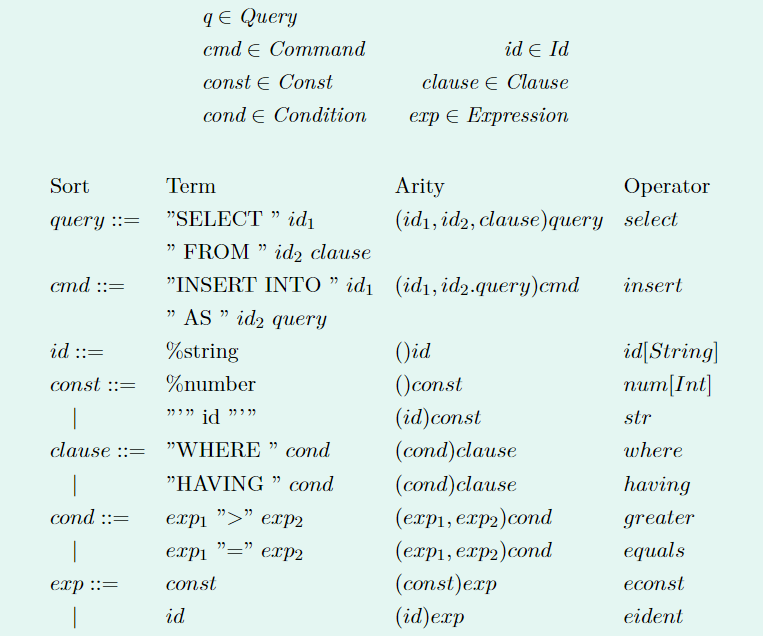
\includegraphics[width=0.5\textwidth]{img/spec-lang-ex.png}
    \end{multicols}

\end{frame}

\begin{frame}[hvid]
    \frametitle{Generic model or code generation?}
    \begin{itemize}
        \item Generic model:
              \begin{itemize}
                  \item No need for code generation (less work and error prone)
                  \item However less efficient and needs thorough well-formedness checks
              \end{itemize}
        \item Code generation:
              \begin{itemize}
                  \item Take advantage of algebraic data types (only well-formed terms can be created)
                  \item However requires code generation
              \end{itemize}
    \end{itemize}
\end{frame}

\begin{frame}[hvid]
    \frametitle{Generating source code}
    \begin{multicols}{2}
        \begin{itemize}
            \item Elm CodeGen package\footfullcite{elm-codegen-package}
            \item Can be useful if integrated with language specification parser
        \end{itemize}
        \columnbreak
        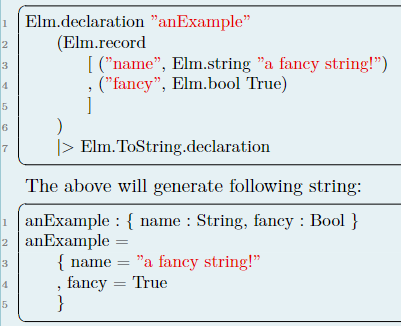
\includegraphics[width=0.4\textwidth]{img/codegen-ex.png}
    \end{multicols}
\end{frame}

\begin{frame}[hvid]
    \frametitle{Generating source code (Continued)}
    \begin{center}
        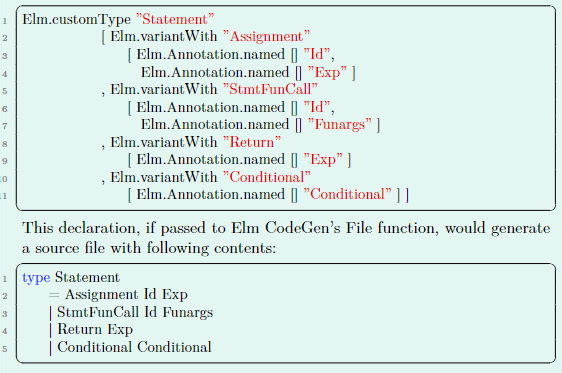
\includegraphics[width=0.5\textwidth]{img/codegen-ex2.png}
    \end{center}
\end{frame}

\begin{frame}[hvid]
    \frametitle{Generating Editor Expression Code}
    \begin{multicols}{2}
        \begin{itemize}
            \item Unique decomposition
                  \begin{itemize}
                      \item Generate a path to the cursor
                      \item Generate an abt of sort $s^C \in \mathcal{S}^C$ based on the path and stop at the cursor
                      \item Generate an abt of sort $\dot{s} \in \dot{\mathcal{S}}$
                            based on the rest of the tree that was not traversed
                  \end{itemize}
        \end{itemize}
        \columnbreak
        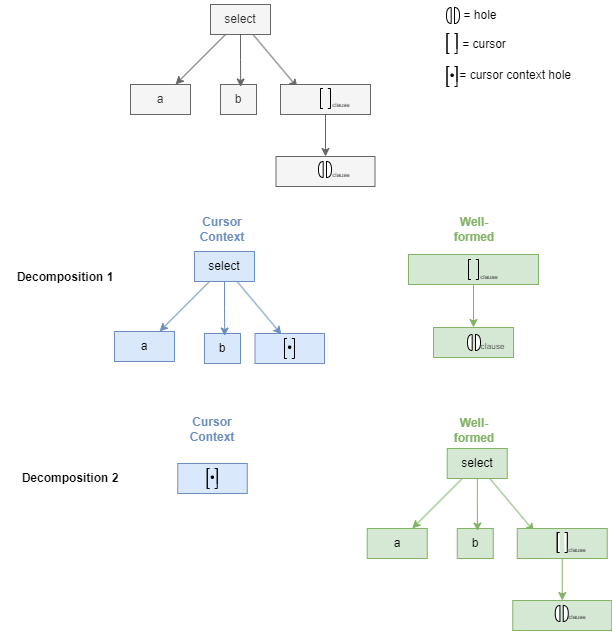
\includegraphics[width=0.4\textwidth]{img/slq-decompose-ex.drawio.png}
    \end{multicols}
\end{frame}

\begin{frame}[hvid]
    \frametitle{Generating Editor Expression Code (Continued)}
    \begin{itemize}
        \item Cursor movement (child and parent)
    \end{itemize}
    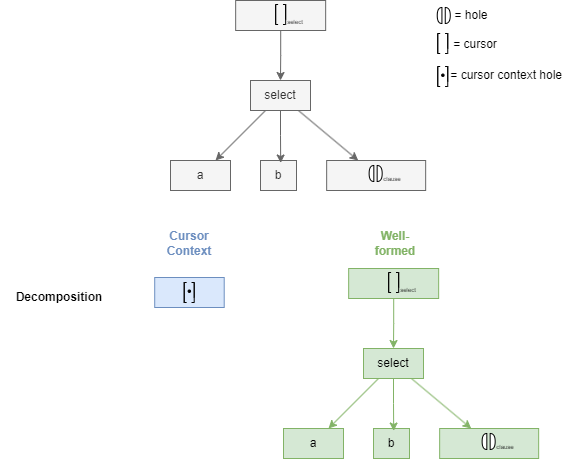
\includegraphics[width=0.3\textwidth]{img/slq-decomp-only.drawio.png}
    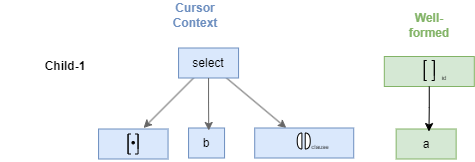
\includegraphics[width=0.3\textwidth]{img/sql-child1.drawio.png}
    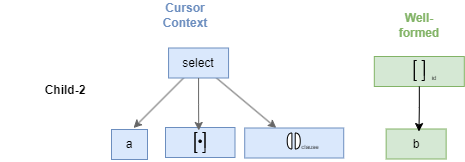
\includegraphics[width=0.3\textwidth]{img/sql-child2.drawio.png}
\end{frame}

\begin{frame}[hvid]
    \frametitle{Generating Editor Expression Code (Continued)}
    \begin{itemize}
        \item Substitution
        \item Conditionals
        \item Sequence
        \item Recursion
    \end{itemize}
\end{frame}


\begin{frame}[hvid]
    \frametitle{Editor examples}
    \begin{itemize}
        \item C
        \item SQL
        \item \LaTeX
    \end{itemize}
\end{frame}


\begin{frame}[hvid]
    \frametitle{C}
    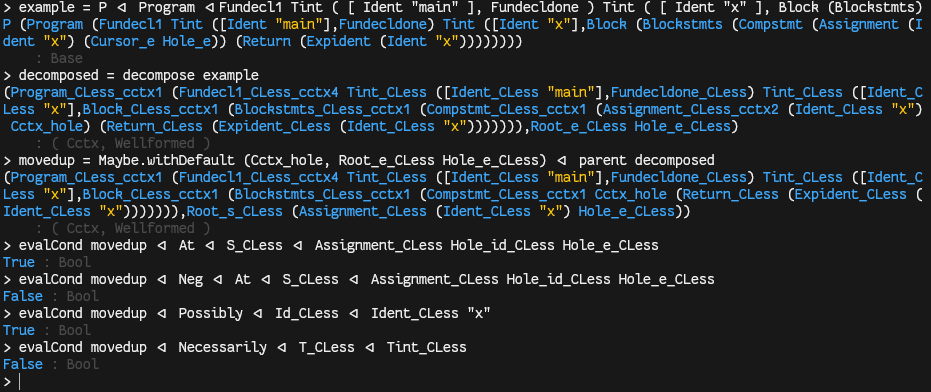
\includegraphics[width=\textwidth]{img/c-repl.png}
\end{frame}

\begin{frame}[hvid]
    \frametitle{SQL}
    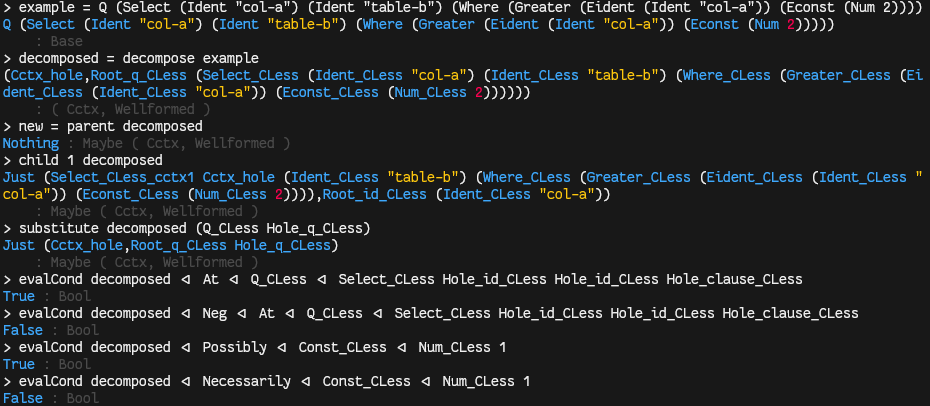
\includegraphics[width=\textwidth]{img/sql-repl.png}
\end{frame}

\begin{frame}[hvid]
    \frametitle{\LaTeX}
    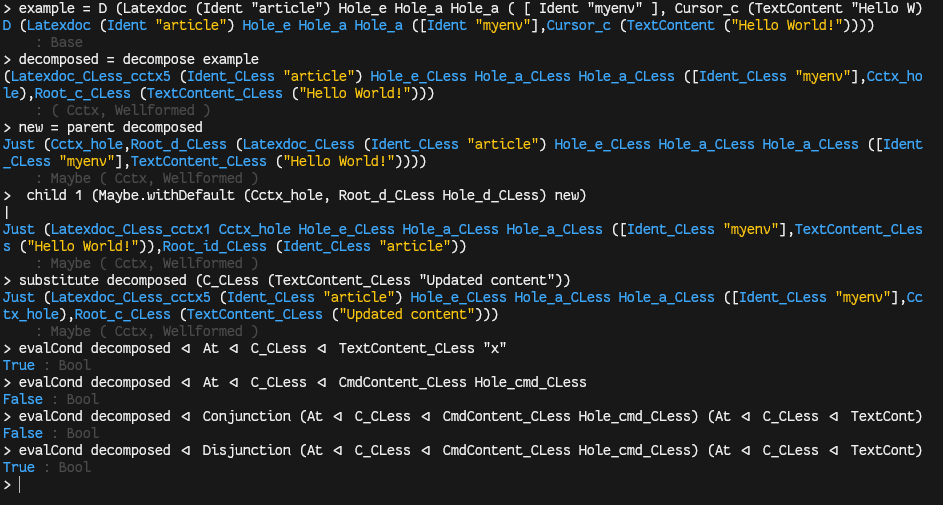
\includegraphics[width=0.9\textwidth]{img/latex-repl.png}
\end{frame}


\begin{frame}[hvid]
    \frametitle{Conclusion of the project}
    \begin{itemize}
        \item<1-> MVP has been achieved
        \item<2-> Some editor expressions are not yet implemented
        \item<3-> Missing criteria for a "good" implementation:
              \begin{itemize}
                  \item Handling context-sensitive syntax
                  \item Views of code being edited
              \end{itemize}
    \end{itemize}
\end{frame}


\begin{frame}[hvid]
    \frametitle{Future work}

    \begin{itemize}
        \item Implement the missing editor expressions
        \item Handling context-sensitive syntax
        \item Views of code being edited
        \item Consider a more concise implementation (maybe in Haskell)
        \item Add support for adding starting symbol to the specification language
    \end{itemize}
\end{frame}



\begin{frame}[hvid]
    \frametitle{Questions}
    \centering
    \large{Thank you for your attention!}
\end{frame}

\end{document}